%
% main.tex -- Paper zum Thema <perturbation>
%
% (c) 2020 Hochschule Rapperswil
%
\chapter{Störungstheorie\label{chapter:perturbation}}
\lhead{Störungstheorie}
\begin{refsection}
\chapterauthor{Daniel Bucher und Thomas Kistler}

%
% einleitung.tex -- Beispiel-File für die Einleitung
%
% (c) 2020 Prof Dr Andreas Müller, Hochschule Rapperswil
%
\section{Einleitung\label{laplace:section:einleitung}}
\rhead{Einleitung}
Lorem ipsum dolor sit amet, consetetur sadipscing elitr, sed diam
nonumy eirmod tempor invidunt ut labore et dolore magna aliquyam
erat, sed diam voluptua \cite{laplace:bibtex}.
At vero eos et accusam et justo duo dolores et ea rebum.
Stet clita kasd gubergren, no sea takimata sanctus est Lorem ipsum
dolor sit amet.

Lorem ipsum dolor sit amet, consetetur sadipscing elitr, sed diam
nonumy eirmod tempor invidunt ut labore et dolore magna aliquyam
erat, sed diam voluptua.
At vero eos et accusam et justo duo dolores et ea rebum.  Stet clita
kasd gubergren, no sea takimata sanctus est Lorem ipsum dolor sit
amet.



%
% problemstellung.tex -- Beispiel-File für die Beschreibung des Problems
%
% (c) 2020 Severin Weiss
%



\section{Motivation: Lösung einer linearen Differentialgleichung
\label{laplace:section:problemstellung}}
\rhead{Problemstellung}
Wir wollen eine Lösung $f(t)$ aus $F(s)$ der linearen Differentialgleichung 
\begin{equation}
\frac{df}{dt} + \lambda f(t) = 0, ~~mit f_{0} = f(t=0)
\end{equation}
Mit der Laplactransformation folgt
\begin{equation}
(sF(s) - f_{0}) + \lambda F(s) = 0.
\label{laplace:dgl}
\end{equation}
Die Gleichung \eqref{laplace:dgl} im Frequenzbereich kann nach $F(s)$ aufgelöst werden.
Es folgt somit
\begin{equation}
F(s) = \frac{f_{0}}{s + \lambda}
\label{laplace:F(s)}
\end{equation}
Um die Laplaceinverse von $F(s)$ zu finden existieren für gewisse Funktionstypen tabellierte zugehörige Rücktransformationen.
Für die Funktion in Gleichung \eqref{laplace:F(s)} $F(s)$ ergibt sich zum Beispiel
\begin{equation}
\mathcal{L}^{-1}\{F(s)\}=\mathcal{L}^{-1}\{\frac{f_{0}}{s+\lambda}\} = f_{0}e^{-\lambda t}
\end{equation}
Solche Tabellen sind jeweils in der Literatur zu finden, welche sich mit der Laplacetransformation beschäftigt.
Wenn für die gegebene Funktion $F(s)$ keine zugehörige Funktion tabelliert ist, muss das Integral \eqref{laplace:riemanninversionsformel} wie in der Einleitung beschrieben numerisch berechnet werden.


\section{Numerische Lösung
\label{perturbation:section:nummerischeloesung}}
\rhead{Nummerische Lösung}
Die Gleichungen \eqref{eq:x_diff} lassen sich durch numerische Verfahren lösen.
Wenn man sich nun jedoch einen Satelliten oder eine Rakete vorstellt, haben diese nur eine begrenzte Rechenkapazität.
Aus diesem Grund wird die komplexere Berechnung durch eine Bodenstation durchgeführt.
Die Resultate der Berechnung werden jeweils dem Flugobjekt mitgeteilt, sodass dieses mit einfacheren Formeln seine Bahn für die nahe Zukunft annähernd abschätzen kann.
Dieses Kapitel beschäftigt sich mit der genaueren, komplexeren Lösung des Problems, welche durch die Bodenstation übernommen wird.

Da das Runge-Kutta-Verfahren nur mit Differentialgleichungen erster Ordnung umgehen kann, muss die Ordnung des Gleichungssystems \eqref{eq:x_diff}  zuerst um eins reduziert werden.
\index{Runge-Kutta-Verfahren}%
Dies kann erreicht werden, indem zwei Hilfsvariablen $v_x = \dot{x}$ und $v_y = \dot{y}$ eingeführt werden.
Das System wird somit um eine Ordnung reduziert, erhält aber im Austausch zusätzliche Dimensionen:
\index{Reduktion der Ordnung}%
\begin{equation*}
\begin{aligned}
	\dot{r_x} &= v_x  \\
	\dot{r_y} &= v_y \\
	\dot{v_x} &= \frac{k}{m} \cdot \sqrt{v_x^2 + v_y^2} \cdot v_x \\
	\dot{v_y} &= \frac{k}{m} \cdot \sqrt{v_x^2 + v_y^2} \cdot v_y - g.
\end{aligned}
\end{equation*}
Als Vektor formuliert:
\[
\frac{d}{dt}\begin{pmatrix}r_x\\r_y\\v_x\\v_y\end{pmatrix} = \begin{pmatrix}v_x\\v_y\\\frac{k}{m} \cdot \sqrt{v_x^2 + v_y^2} \cdot v_x\\\frac{k}{m} \cdot \sqrt{v_x^2 + v_y^2} \cdot v_y - g\end{pmatrix}.
\]

Damit haben wir eine mit dem  Runge-Kutta-Verfahren lösbare Variante der Differentialgleichung gefunden.
Der Python Code in Listing \ref{buch:listing:diffprogram} löst die Differentialgleichung mit Hilfe der Library \textit{SciPy}.
\index{Python}%
\index{ScyPi@\textit{SciPy}}
Die Bodenstation, die zu komplexen Berechnungen in der Lage ist,
führt also in einem regelmässigen Zeitintervall die Funktion \texttt{runge\_kutta(t)}
auf dem Differentialgleichungssystem aus und erhält so die Position und die Geschwindigkeit zu einem bestimmten Zeitpunkt.


\lstinputlisting[style=Python,float,caption={Programm zur
	Berechnung des Differentialgleichungssystems},label={buch:listing:diffprogram}]{papers/perturbation/diffsolution.py}


\section{Erster Lösungsansatz
\label{perturbation:section:ersterloesungsansatz}}
\rhead{Erster Lösungsansatz}

Die Formeln \ref{eq:x_simple} und \ref{eq:y_simple} sind ohne viel Rechenleistung berechenbar und somit auch als Flugobjekt durchführbar. Die Störungstheorie befasst sich damit, die Starparameter $x_0$, $y_0$, $v_{0_x}$ und $v_{0_y}$ so abzuändern, dass dennoch gute Approximationen für $x(t)$ und $y(t)$ gefunden werden können. Hierbei ist es die Aufgabe der Bodenstation, die notwendigen Startparameter dem Flugobjekt mitzuteilen, sodass dieses die Berechnung auf Basis der trivialen Formeln \ref{eq:x_simple} und \ref{eq:y_simple} vornehmen kann.

Als ersten Lösungsansatz haben wir $v_{0_x}$ und $v_{0_y}$ durch lineare Funktionen abhängig von der Zeit ersetzt, aber $x_0$ und $y_0$ vorerst unberührt gelassen. Hintergrund dieser Überlegung ist, dass der Luftwiderstand ja nur die Geschwindigkeit beeinflusst.
\[
v_{0_x} \rightarrow v_{0_x}(t) = v_{0_x} + \nu_x \cdot t
\]
\[
v_{0_y} \rightarrow v_{0_y}(t) = v_{0_y} + \nu_y \cdot t
\]

Wir passen die Startgeschwindigkeit im Verlaufe der Zeit $t$ also anhand eines unbekannten Faktors $\nu$ an. Eingesetzt in die Formeln \ref{eq:x_simple} und \ref{eq:y_simple} erhalten wir:
\begin{equation}\label{eq:x_linear}
    x(t) = x_0 + t \cdot (v_{0_x} + \nu_x \cdot t)
\end{equation}
\begin{equation}\label{eq:y_linear}
    y(t) = y_0 + t \cdot (v_{0_y} + \nu_y \cdot t) - \frac{1}{2}gt^2
\end{equation}

$x_0$, $y_0$, $v_{0_x}$ und $v_{0_y}$ sind die bekannten Anfangsbedingungen des Problems. Ebenfalls können $x(t)$ und $y(t)$ mit dem Runge Kutta Verfahren bestimmt werden, wie in Kapitel \ref{chapter:numerische_lsg} beschrieben. Um neue Werte mit der Störung zu bestimmen, müssen die Unbekannten $\nu_x$ und $\nu_y$ berechnet werden. Diese können bestimmt werden, in den man die Gleichungen \ref{eq:x_linear} und \ref{eq:y_linear} nach $\nu_x$ bzw. $\nu_y$ auflöst:
\[
\nu_x = \frac{x(t) - x_0 - tv_{0_x}}{t^2}
\]
\[
\nu_y = \frac{y(t) - y_0 - tv_{0_y} + \frac{1}{2}gt^2}{t^2}
\]

Beispielsweise kann dieses Gleichungssystem für $t = 5s$ gelöst werden. Dadurch erhält man $\nu_x$ und $\nu_y$. Da hierzu allerdings $x(t=5)$ und $y(t=5)$ mittels Runge-Kutta berechnet werden müssen, ist dazu nur die Bodenstation in der Lage. Die Werte $\nu_x$ und $\nu_y$ können nun aber dem Flugobjekt übertragen werden, welches mit den Formeln \ref{eq:x_linear} und \ref{eq:y_linear} seine Position in naher Zukunft nun autonom approximieren kann, beispielsweise für das Intervall $t \in [5,6)$. Anschliessend könnte die Bodenstation die Werte $\nu_x$ und $\nu_y$ für $t=6s$ neu berechnen, um den Fehler nicht beliebig anwachsen zu lassen.

Geplottet ergibt dies das Resultat in Abbildung \ref{naive_linear_term}. Rot ist das dabei das nummerische Resultat der Differentialgleichungen \ref{eq:x_diff} und \ref{eq:y_diff}, blau ohne eingesetzte lineare Funktion und türkis die korrigierte Variante. Für die korrigierte Variante wurde eine Intervalllänge von $t=1s$ gewählt. Das heisst, sie bestimmt die Unbekannten $\nu_x$ und $\nu_y$ zu jeder vollen Sekunde $t \in \{1, 2, 3, \cdots, 25\}$ und nutzt jene Daten, um die Position jeweils eine Sekunde später vorherzusagen. Wie zu erkennen ist kann ein Grossteil des Fehlers bereits vermieden werden.
\begin{figure}
    \centering
    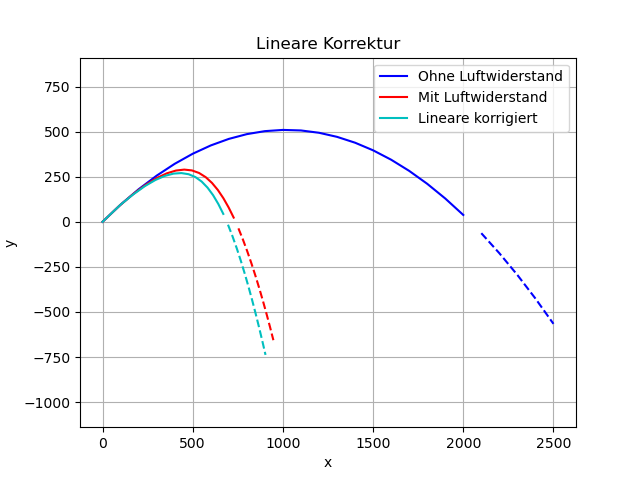
\includegraphics[scale=0.7]{papers/perturbation/bilder/img1.png}
    \caption{Linearer Korrekturterm}
	\label{naive_linear_term}
\end{figure}


Anstelle des linearen Ansatzes könnte man auch einen quadratischen Ansatz nutzen. Dies ergibt anstelle von \ref{eq:x_linear} und \ref{eq:y_linear}:
\begin{equation}
    x(t) = x_0 + t \cdot (v_{0_x} + \nu_{x_1}t + \nu_{x_2}t^2) = x_0 + v_{0_x}t + \nu_{x_1}t^2 + \nu_{x_2}t^3
\end{equation}
\begin{equation}
    y(t) = y_0 + t \cdot (v_{0_y} + \nu_{y_1}t + \nu_{y_2}t^2) - \frac{1}{2}gt^2 = y_0 + v_{0_y}t + \nu_{y_1}t^2 + \nu_{y_2}t^3 - \frac{1}{2}gt^2
\end{equation}

Damit haben wir noch bessere Resultate erhalten. Diese sind in Abbildung \ref{naive_quadratic_term} ersichtlich. Von Auge ist bereits kein Unterschied der beiden Flugbahnen mehr erkennbar.
\begin{figure}
    \centering
    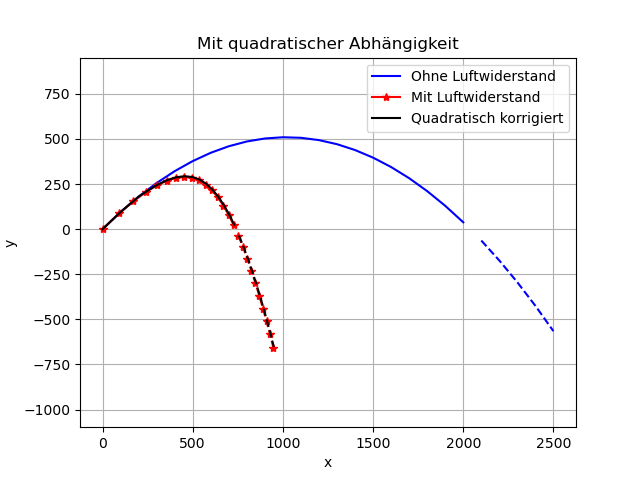
\includegraphics[scale = 0.7]{papers/perturbation/bilder/img2.png}
    \caption{Quadratischer Korrekturterm}
	\label{naive_quadratic_term}
\end{figure}
\section{Verbesserte Lösung
\label{perturbation:section:verbesserte_loesung}}
\rhead{Verbesserte Lösung}

Anstelle lediglich den Anfangswert $\vec{v_0}$ anzupassen, erhält man bessere Resultate, indem auch $\vec{r_0} = (x_0, y_0)$ variabel gestaltet wird.
Zudem kann man anstelle von $t$ nur die Differenz $\Delta t$ seit dem letzten Update von der Bodenstation betrachten.

Wiederum ist das Ziel, dass der Flugkörper mit den einfachen Formeln \eqref{eq:x_simple} eine möglichst gute Approximation auf einfache Art und Weise berechnen kann,
indem er die Anfangswerte $\vec{r_0}$ und $\vec{v_0}$ im Laufe der Zeit gemäss Weisungen der Bodenstation anpasst.

In einem ersten Schritt verlangen wir von der Bodenstation, welche $\vec{r}$, aber auch $\vec{v}$ mit dem Runge Kutta Verfahren berechnen kann,
eben diese Werte um so eine Approximation mit den simplen Formeln \eqref{eq:x_simple} tätigen zu können.
Es ergeben sich folgende Formeln:

\begin{equation}
\begin{aligned}
x(t + \Delta t) &= x_0 + v_{0x}\Delta t\\
y(t + \Delta t) &= y_0 + v_{0y}\Delta t - \frac{1}{2}g\Delta t^2
\end{aligned}
\end{equation}

Verlangt man von der Bodenstation jede Sekunde neue Werte für die Elemente $x_0, y_0, v_{0x}$ und $v_{0y}$ gibt dies eine Genauigkeit von 2 Stellen.
In Abbildung \ref{error} ist der Fehler ersichtlich.
Dieser ist als euklidische Distanz zur effektiven Position dargestellt.

\begin{figure}
    \centering
    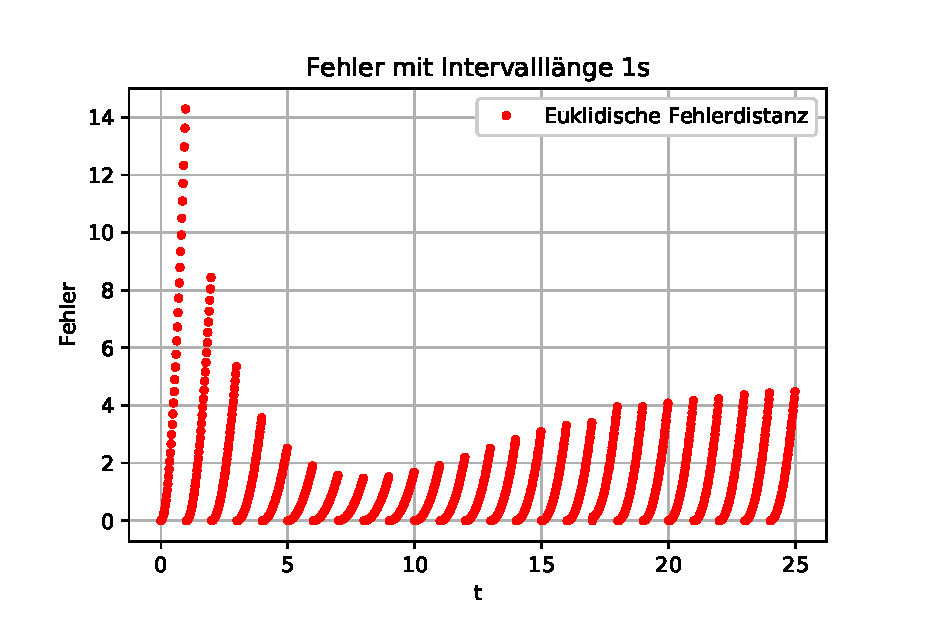
\includegraphics[scale = 0.7]{papers/perturbation/bilder/perturbation_fig3.eps}
    \caption{Fehler als euklidische Distanz}
	\label{error}
\end{figure}
\section{Möglichkeiten zur Genauigkeitssteigerung
\label{perturbation:section:weitereverbesserungen}}
\rhead{Weitere Verbesserungen}
In diesem Abschnitt diskutieren wir Verbesserungsmöglichkeiten, um den Fehler weiter zu minimieren.
Abbildung \ref{error} zeigt, dass der Fehler stark von der Intervalllänge abhängt.
Eine Reduktion der Intervalllänge beschreiben wir im nächsten Abschnitt.
Weiter lassen sich mit Hilfe der Störungstheorie höherer Ordnung genauere Resultate erzielen.

\subsection{Reduktion der Intervalllänge}
In Abbildung \ref{error} ist der Fehler für die Intervalllänge von einer Sekunde ersichtlich.
Wie man erkennen kann, nimmt dieser innerhalb eines solchen Intervalls stark zu.
Dies ist vor allem unserem Beispiel geschuldet, da die Störung (in unserem Beispiel der Luftwiderstand) kurzfristig eine grosse Auswirkung auf das Resultat hat.
Bei Berechnungen von z.B. Satellitenbahnen wäre dies anders, da Störungen,
wie die Gravitation von Planeten, viel kleiner sind und die Abweichungen erst bei längeren Intervalldauern auftreten.

Für unser Beispiel haben wir in einem ersten Schritt die Intervalllänge halbiert.
Daraus resultierte der Fehler in Abbildung \ref{errorShortInterval}.
Wie ersichtlich ist, ist der Fehler um ca. Faktor 4 kleiner.
Wir erhalten somit weitere 2 Bit Genauigkeitsgewinn.
Weiter ist zum Zeitpunkt $t=17s$ eine kleine numerische Instabilität beobachtbar.

\begin{figure}
    \centering
    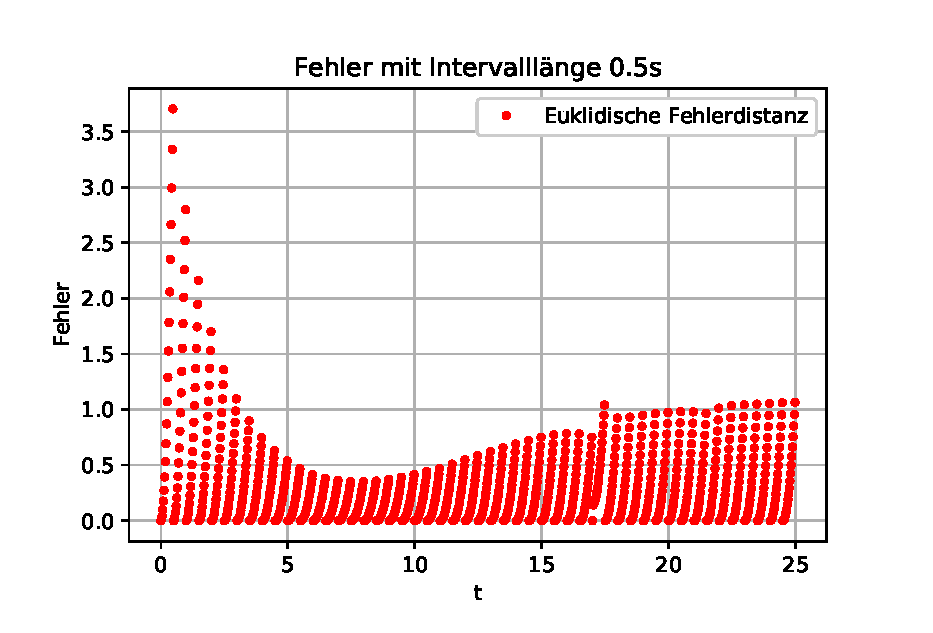
\includegraphics[scale=0.7]{papers/perturbation/bilder/perturbation_fig4.eps}
    \caption{Fehler bei halbierter Intervalldauer}
	\label{errorShortInterval}
\end{figure}

In einem zweiten Schritt haben wir die Intervalllänge nochmals auf die Länge $0.25s$ halbiert.
Dies ist in Abbildung \ref{errorShortInterval2} ersichtlich.
Wir erhalten erneut einen Genauigkeitsgewinn um den Faktor 4 bzw. 2 Bit.
Dies lässt sich leider jedoch nicht weiter beliebig fortsetzen.
Die Rechenlast des Satelliten bleibt konstant und ist nicht von der Intervalllänge abhängig.
Der Aufwand für die Bodenstation nimmt jedoch zu.
Die numerischen Berechnungen für aufwendige Probleme (wie z.B. Satellitenbahnen) benötigen auch für die Bodenstation viel Rechenleistung und
können nicht beliebig oft ausgeführt werden.

\begin{figure}
    \centering
    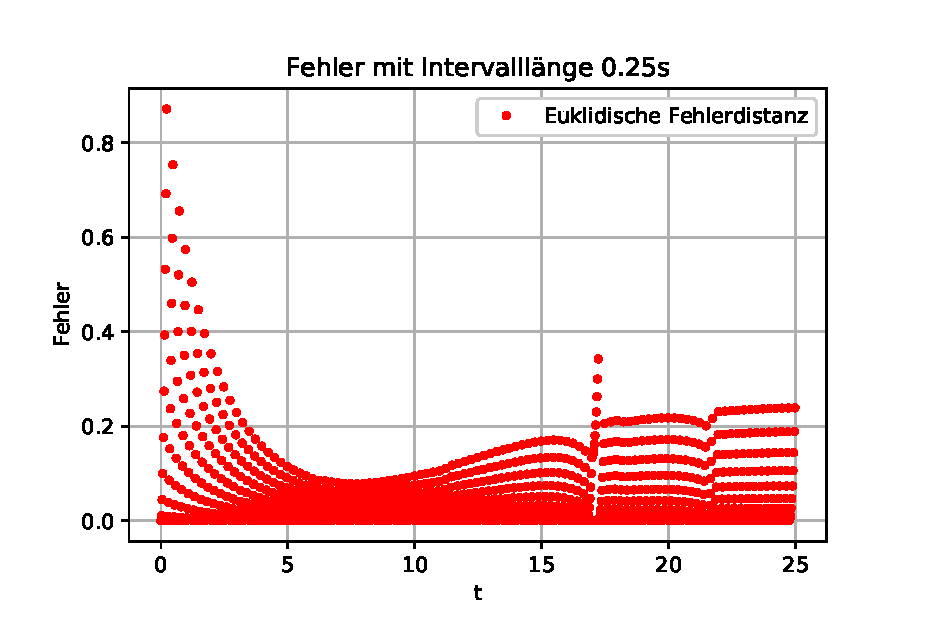
\includegraphics[scale=0.7]{papers/perturbation/bilder/perturbation_fig5.eps}
    \caption{Fehler mit einem Viertel der ursprünglichen Intervalldauer}
	\label{errorShortInterval2}
\end{figure}

\subsection{Erhöhung der Ordnung}
Eine andere Möglichkeit zur Steigerung der Genauigkeit eröffnet sich dadurch, dass man anstelle $x_0, y_0, v_{0x}$ und $v_{0y}$,
was an sich Polynome nullter Ordnung sind, Polynome höherer Ordnung ansetzt.
Wir schauen uns ein Beispiel erster Ordnung an.
Wir ändern nun die Anfangsbedingungen folgendermassen.
Um die Notation klar zu halten, werden wir nicht länger $x_0$ und $y_0$ verwenden, sondern vom Ortsvektor $\vec{r_0}$ sprechen.

\begin{equation}
\label{eq:ordnung1_linear_ansatz}
\begin{aligned}
x_0 &\longrightarrow \textcolor{red}{r_{x0} +  r_{x1}  \cdot \Delta t}\\
y_0 &\longrightarrow \textcolor{red}{r_{y0} +  r_{y1}  \cdot \Delta t}\\
v_x &\longrightarrow \textcolor{blue}{v_{x0} + v_{x1}  \cdot \Delta t}\\
v_y &\longrightarrow \textcolor{blue}{v_{y0} + v_{y1}  \cdot \Delta t}\\
\end{aligned}
\end{equation}

Betrachten wir nun ein bestimmtes Intervall, etwa $t \in [5,6)$.
Innerhalb dieses Intervalls arbeiten wir mit $t=5$, $\Delta t \in [0,1)$.
$t$ wird also fixiert und $\Delta t$ ist unsere neue Variable.
So gilt nach Einsetzen in Gleichungen \eqref{eq:x_simple} 

\begin{equation}\label{eq:ordnung1_linear_r}
\begin{aligned}
r_x(t + \Delta t) &= \textcolor{red}{(r_{x0} +   r_{x1} \cdot \Delta t)} + \textcolor{blue}{(v_{x0} + v_{x1}  \cdot \Delta t)} \cdot \Delta t \\
r_y(t + \Delta t) &= \textcolor{red}{(r_{y0} +   r_{y1} \cdot \Delta t)} + \textcolor{blue}{(v_{y0} + v_{y1} \cdot \Delta t)} \cdot \Delta t - \frac{1}{2}g \Delta t^2
\end{aligned}
\end{equation}

Um das Problem lösen zu können, werden wir vorerst eine exklusive Betrachtung der Geschwindigkeit durchführen.
Indem man Gleichung \ref{eq:x_simple} nach $t$ ableitet und anschliessend unseren Ansatz für die Anfangsbedingungen einsetzt, erhält man

\begin{equation}\label{eq:ordnung1_linear_v}
\begin{aligned}
v_x(t + \Delta t) &= \textcolor{blue}{(v_{x0} + v_{x1}  \cdot \Delta t)} \\
v_y(t+ \Delta t) &= \textcolor{blue}{(v_{y0} + v_{y1} \cdot \Delta t)} - g \Delta t
\end{aligned}
\end{equation}

\subsubsection{Lösung des Problems mit linearer Interpolation}
\label{section:perturbation_ordnung1_linear}

In obigen Gleichungen sind die acht Unbekannten $r_{x0}, r_{x1}, r_{y0}, r_{y1}, v_{x0}, v_{x1}, v_{y0}$ und $v_{y1}$ zu bestimmen.
Zwar haben wir mit Gleichungen \ref{eq:ordnung1_linear_r} und \ref{eq:ordnung1_linear_v} nur vier Gleichungen zur Verfügung,
indem wir aber $\Delta t$ variieren, können wir die Anzahl Gleichungen beliebig erhöhen.
Das Gleichungssystem ist somit lösbar.
Wir machen uns hierbei zu Nutze, dass die Bodenstation mit dem Runge-Kutta-Verfahren $\vec{r}(t + \Delta t)$ und $\vec{v}(t + \Delta t)$ liefern kann.
Dies sind also bekannte Werte, unabhängig davon, wie $\Delta t$ gesetzt wird.\\

Indem wir $\Delta t = 0$ setzen, erhalten wir auf relativ einfache Art und Weise all jene Unbekannten, die mit einer $0$ indiziert sind.
Wir nutzen hierbei Gleichung \eqref{eq:ordnung1_linear_r} zur Bestimmung von $\vec{r_0}$, und Gleichung \eqref{eq:ordnung1_linear_v} zur Bestimmung von $\vec{v_0}$.

\begin{equation}
\label{eq:ordnung1_linear_solutionPart1}
\begin{aligned}
r_{x0} &= r_x(t) \\
r_{y0} &= r_y(t) \\
v_{x0} &= v_x(t) \\
v_{y0} &= v_y(t) \\
\end{aligned}
\end{equation}

Um $v_{x1}$ und $v_{y1}$ zu bestimmen, können wir nun weiterhin Gleichung \ref{eq:ordnung1_linear_v} verwenden, müssen aber das $\Delta t$ alternieren.
Für eine lineare Interpolation bietet sich $\Delta t = 1s$ an.
Man könnte aber auch z.B. die halbe Intervalldauer $\Delta t = 0.5s$ wählen.
Mit einer einfachen Umformung ergibt sich:

\begin{equation}
\label{eq:ordnung1_linear_solutionPart2}
\begin{aligned}
v_{x1} &=  \frac{v_x(t + \Delta t) - v_{x0}}{\Delta t} \\
v_{y1} &=  \frac{v_y(t + \Delta t) - v_{y0} + g \cdot t}{\Delta t}
\end{aligned}
\end{equation}

Wie zu erkennen ist, machen wir bereits Gebrauch von den zuvor bestimmten Unbekannten.
Zu guter Letzt können mit Gleichung \ref{eq:ordnung1_linear_r} die zwei verbleibenden Unbekannten bestimmt werden:

\begin{equation}
\label{eq:ordnung1_linear_solutionPart3}
\begin{aligned}
r_{x_1} &= \frac{r_x(t + \Delta t) - r_{x0} - \Delta t \cdot(v_{x0} + v_{x1}  \cdot \Delta t)}{\Delta t} \\
r_{y_1} &= \frac{r_y(t + \Delta t) - r_{y0} - \Delta t \cdot(v_{y0} + v_{y1}  \cdot \Delta t) + 0.5gt^2}{\Delta t}
\end{aligned}
\end{equation}


Somit sind nun alle Unbekannten bestimmt und Gleichung \eqref{eq:ordnung1_linear_r} kann zur Bestimmung des Ortes herangezogen werden.
Berechnen wir die Position schrittweise für die Intervalle $\{[0,1), [1, 2), \dots\}$ ergibt sich die euklidische Fehlerdistanz in Bild \ref{fig:ordnung1_linear_error_A}.

Anstelle der Interpolation an den Stützstellen $\Delta t = 0$ und $\Delta t = 1$ liessen sich, wie bereits erwähnt, auch die Stützstellen $\Delta t = 0$ und $\Delta t = 0.5s$ nutzen.
Dies führt zu der Fehlerverteilung gemäss Bild \ref{fig:ordnung1_linear_error_B}.

In beiden Grafiken ist schön zu erkennen, wie der Fehler jeweils bei einer Stützstelle auf $0$ sinkt, zwischen den Stützstellen aber einen Anstieg verzeichnet.
Es ist auch gut zu erkennen, dass die Wahl der Stützstellen jeweils am Anfang und am Ende erfolgen sollte, um einen maximalen Bereich des Intervalls abzudecken.

Vergleichen wir den Fehler aus Grafik \ref{fig:ordnung1_linear_error_A} mit Polynomen nullter Ordnung in Grafik \ref{error} erkennen wir erneut eine Genauigkeitssteigerung um Faktor vier.
Die Erhöhung der Ordnung um eins hat also den selben Effekt wie wie Halbierung der Intervalldauer.

Selbstverständlich könnte der Anwender auch beide Verfahren kombinieren.
Der Fehler davon ist in Grafik \ref{fig:ordnung1_linear_error_C} abgebildet.
Erneut ist er viermal kleiner geworden.
Die Abweichung beträgt nun kaum noch mehr als $1m$.

\begin{figure}
	\centering
	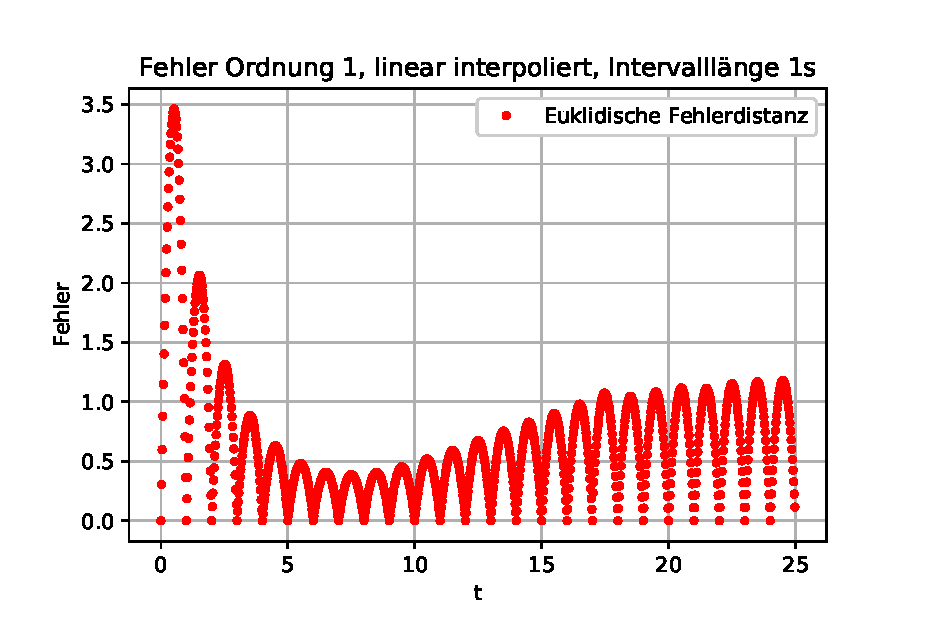
\includegraphics[scale=0.7]{papers/perturbation/bilder/perturbation_fig6.eps}
	\caption{Fehler bei Polynomen erster Ordnung}
	\label{fig:ordnung1_linear_error_A}
\end{figure}

\begin{figure}
	\centering
	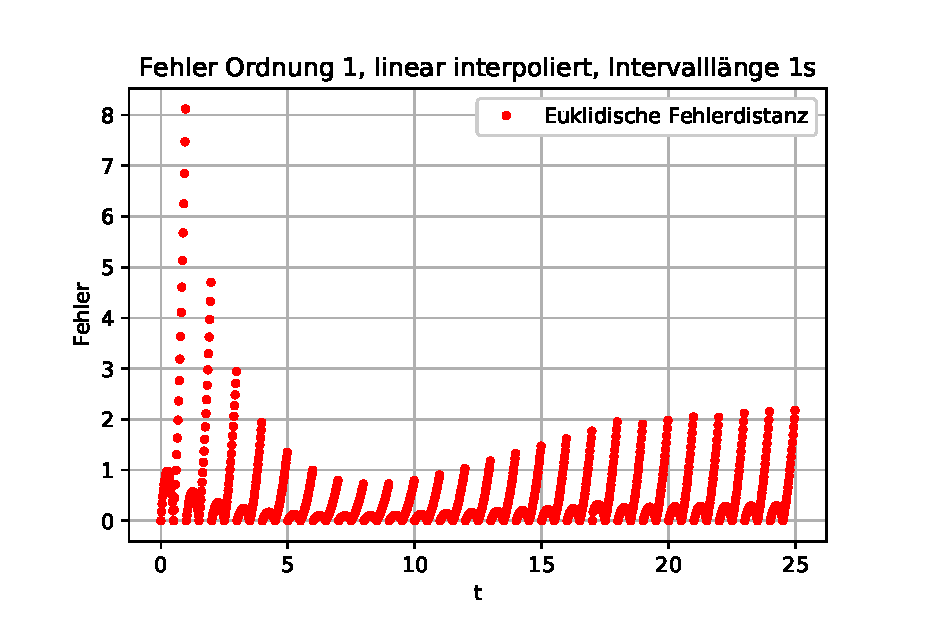
\includegraphics[scale=0.7]{papers/perturbation/bilder/perturbation_fig7.eps}
	\caption{Fehler bei Polynomen erster Ordnung mit variierten Stützstellen}
	\label{fig:ordnung1_linear_error_B}
\end{figure}

\begin{figure}
	\centering
	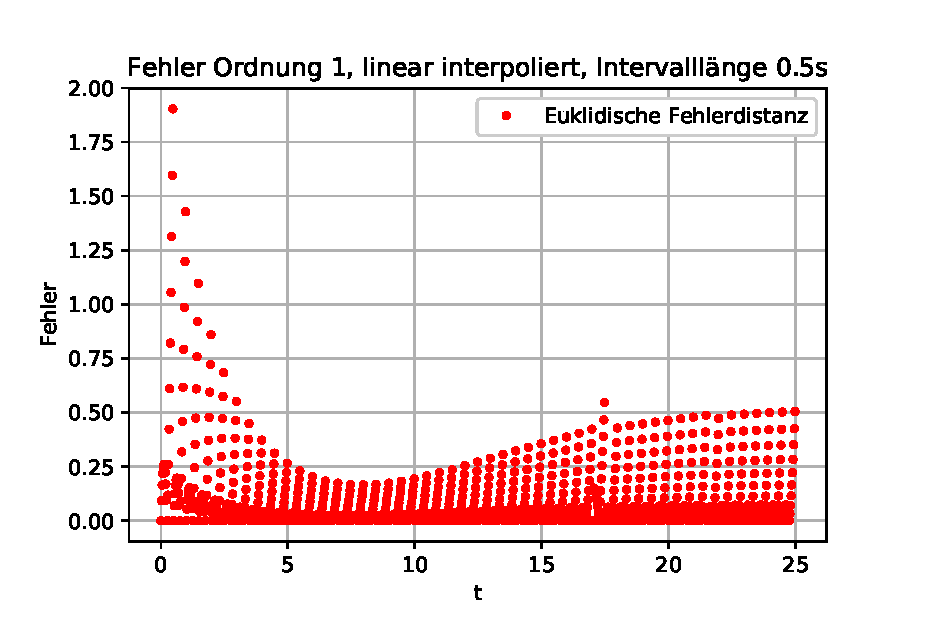
\includegraphics[scale=0.7]{papers/perturbation/bilder/perturbation_fig8.eps}
	\caption{Fehler bei Polynomen erster Ordnung mit halbierter Intervalldauer}
	\label{fig:ordnung1_linear_error_C}
\end{figure}

\subsubsection{Lösung des Problems mit Taylorreihen}
Anstelle von linearer Interpolation kann man die Unbekannten $r_{x0}, r_{x1}, r_{y0}, \dots$ auch mit anderen Verfahren bestimmen.
Wir können den Ansatz \eqref{eq:ordnung1_linear_ansatz} als Taylorentwicklungen interpretieren.
Betrachten wir nur die Ortskoordinate und leiten wir diese nach $\Delta t$ ab, erhalten wir das folgende System.
Um die Notation kurz zu halten, verwenden wir Vektornotation anstelle der Aufteilung nach $x$- und $y$-Komponenten.

\begin{equation}
\label{eq:ordnung1_taylor_ansatz}
\begin{aligned}
\vec{r} &=  \vec{r_0} + \vec{r_1} \cdot \Delta t \\
\vec{\dot{r}} &= \vec{r_1} \\
\end{aligned}
\end{equation}

Die Unbekannte $\vec{r_0}$ ist erneut durch setzen von $\Delta t = 0$ sehr einfach zu erlangen, analog zu Kapitel \ref{section:perturbation_ordnung1_linear}.
$\vec{r_1}$ kann ebenfalls ohne grossen Aufwand bestimmt werden, indem wir die Ableitung mit Hilfe der Bodenstation wie folgt annähern:
\[
\vec{\dot{r}}(t) \approx \frac{\vec{r}(t+\epsilon) - \vec{r}(t)}{\epsilon}
\]

Damit ist bereits eine Annäherung des Ortes möglich.
Analog könnte man auch die Geschwindigkeit betrachten.

Beide Varianten, Interpolation und Taylorentwicklung, sind legitim.
Die Interpolation ist am Anfang und Ende des Intervalls exakt, hat dafür aber in der Mitte einen relativ hohen Fehler.
Die Taylorentwicklung ist vor allem zu Beginn des Intervalls exakt.
Dies, da insbesondere bei höheren Ordnungen auch die Krümmung des Kurvenverlaufs berücksichtigt wird.
Da sich allerdings alle Stützstellen am Anfang des Intervalls befinden, wird der Kurvenverlauf zum Ende des Intervalls hin immer ungenauer.

\section{Fazit}
Durch das Studium der Störungstheorie haben wir gesehen, dass auch komplexe Bahnverläufe mit begrenzter Rechenleistung sehr gut approximiert werden können.
Man benötigt allerdings eine Bodenstation, die fähig ist, exakte Werte an vorgegebenen Stützstellen zu berechnen.
Dies kann mit Hilfe numerischer Verfahren zur Lösung komplexer Differentialgleichungen erreicht werden, wie beispielsweise dem Runge-Kutta Verfahren.
Es lassen sich somit Verfahren kreieren, sodass auch ein Satellit oder ein anderes Objekt mit begrenzter Rechenleistung die Bahn approximieren kann.
Dies, obwohl die Bahn von hunderten planetarischen Objekten gestört wird.
Es ist dabei möglich, die Genauigkeit nahezu beliebig zu erhöhen, indem man entweder die Bodenstation in kürzeren Intervallen um neue Werte bittet,
oder Polynome höherer Ordnung anstelle der Anfangswerte einsetzt.

\printbibliography[heading=subbibliography]
\end{refsection}
